%\documentclass[notes,10pt,aspectratio=169]{beamer}

\documentclass[notes, 10pt,aspectratio=169]{beamer}

% Add this line to your preamble
\setbeameroption{show notes on second screen=right}

%\usetheme{Singapore} %Boadilla, Madrid, default, etc. 
\usetheme[progressbar=frametitle]{metropolis}
\usecolortheme{rose} %beaver, dolphin, crane, 


%\setbeamersize{text margin left=4mm, text margin right=4mm}


\usecolortheme{default}

\usepackage[utf8]{inputenc}
\usepackage[T1]{fontenc}
\usepackage{lmodern}
\usepackage{xcolor}
\usepackage{tikz}
\usetikzlibrary{shapes.geometric, arrows, positioning}

\tikzstyle{block} = [rectangle, draw, text width=4cm, align=center, rounded corners, minimum height=1cm]
\tikzstyle{decision} = [rectangle, draw, text width=5cm, align=center, fill=blue!10, rounded corners, minimum height=1cm]
\tikzstyle{terminal} = [rectangle, draw, text width=4.5cm, align=center, fill=yellow!30, rounded corners, minimum height=1cm]
\tikzstyle{end} = [rectangle, draw, text width=5cm, align=center, fill=green!30, rounded corners, minimum height=1cm]
\tikzstyle{arrow} = [->, thick]



\usepackage{adjustbox}
%2. change the bullets 
\setbeamertemplate{itemize item}[triangle] %circle, square,... 


% 1. Define custom colors and set colors 
%\definecolor{myblue}{HTML}{003366}
\definecolor{accent}{RGB}{78,205,196}

%\setbeamercolor{title}{fg=white,bg=myblue}
\setbeamercolor{frametitle}{fg=black,bg=white}
%\setbeamercolor{normal text}{fg=mygray}
\setbeamercolor{block title}{fg=black,bg=blue}
%\setbeamercolor{block body}{fg=black,bg=white}

\setbeamercolor{item}{fg= orange!80} % Change bullet color
\setbeamercolor{button}{bg=orange, fg=white}





% 3. BibLaTeX settings
\usepackage[
  backend=biber,
  style=apa,
  citestyle=authoryear
]{biblatex}
\addbibresource{references.bib}

\title{Centralized Annuities System}
%\subtitle{A Mini Literature Overview}

\author{%
 Lucas Condeza
\inst{1} \and
   %\and
%  Coauthor Three\inst{3}
}
\institute{
  \inst{1} Yale University \\
}

\date{\today}

\begin{document}

\begin{frame}
  \titlepage
\end{frame}

\begin{frame}{Feedback}

\begin{itemize}
    \item I do not like the term aftermarket 
    \item Difficult to model insurance: ignore it?  
\end{itemize}

    
\end{frame}

\begin{frame}{Research question}
    
\begin{itemize}
    
    %Your first slide should have one sentence on it, with a question mark at the end: your research question. Your presentation should start with 5 minutes of discussion about why this is an interesting economics question
    \item What is the impact of aftermarkets (search + bargaining)? 

    \begin{itemize}

    \item Sellers bid, buyers buy or search and bargain 
    
    \item Examples: car dealership, housing market (e.g. Zillow) 

    \item Benchmarks: only bargaining, sellers set prices, aftermarket. 
    
    \end{itemize}

    \item How to model assymetric competition in selection markets? 
\end{itemize}
\end{frame}


\begin{frame}{Research question (version 2)}
    
\begin{itemize}
    
    %Your first slide should have one sentence on it, with a question mark at the end: your research question. Your presentation should start with 5 minutes of discussion about why this is an interesting economics question
    \item What is the impact of aftermarkets? 

    \begin{itemize}

    \item \textbf{What are aftermarkets?} Sellers bid prices then buyers either buy at bidded price or search a seller and bargain. 
    
    \item \textbf{Relevance}: car dealership, housing market (e.g. Zillow), firms hiring workers, and annuities market in Chile

    \item \textbf{Benchmarks}: only bargaining, sellers set prices, aftermarket. 
    
    \end{itemize}
    \begin{figure}
        \begin{adjustbox}{width=\textwidth, center} % This scales everything inside to fit
            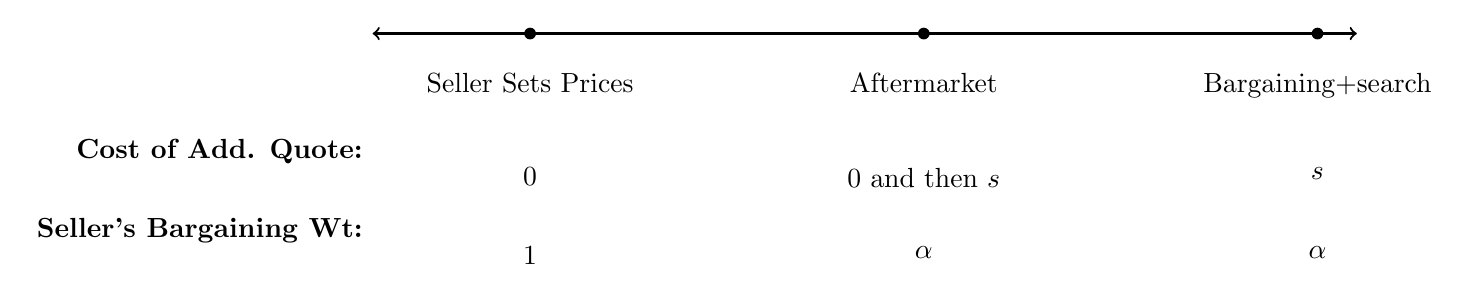
\begin{tikzpicture}[node distance=1cm]
                % Your original TikZ code is here. No changes needed inside.
                \draw[<->, thick] (0,0) -- (12.5,0);
                \node (left) at (2,0) [circle, fill=black, inner sep=1.5pt] {};
                \node (mid) at (7,0) [circle, fill=black, inner sep=1.5pt] {};
                \node (right) at (12,0) [circle, fill=black, inner sep=1.5pt] {};
                \node[anchor=east, align=right] at (0, -1.5) {\textbf{Cost of Add. Quote:}};
                \node[anchor=east, align=right] at (0, -2.5) {\textbf{Seller's Bargaining Wt:}};
                \node[below=1.5cm of left] {$0$};
                \node[below=1.5cm of mid, align=center] {$0$ and then $s$};
                \node[below=1.5cm of right] {$s$};
                \node[below=2.5cm of left] {$1$};
                \node[below=2.5cm of mid] {$\alpha$};
                \node[below=2.5cm of right] {$\alpha$};
                \node[below=0.3cm of left, align=center] {Seller Sets Prices};
                \node[below=0.3cm of mid, align=center] {Aftermarket};
                \node[below=0.3cm of right, align=center] {Bargaining+search};
            \end{tikzpicture}
        \end{adjustbox}
        %\caption{A continuum of market structures based on seller bargaining power and quoting prices.}
        \label{fig:market_continuum_scaled}
         
    \end{figure}
\note{In relevance mention that in Chile there was discussion about the aftermarket and they removed it. 

}
    %\item How to model assymetric competition in selection markets? 
\end{itemize}
\end{frame}




 
%%%%%%%%%


\begin{frame}
\frametitle{Different use of the aftermarket} 
\begin{figure}
    \centering
    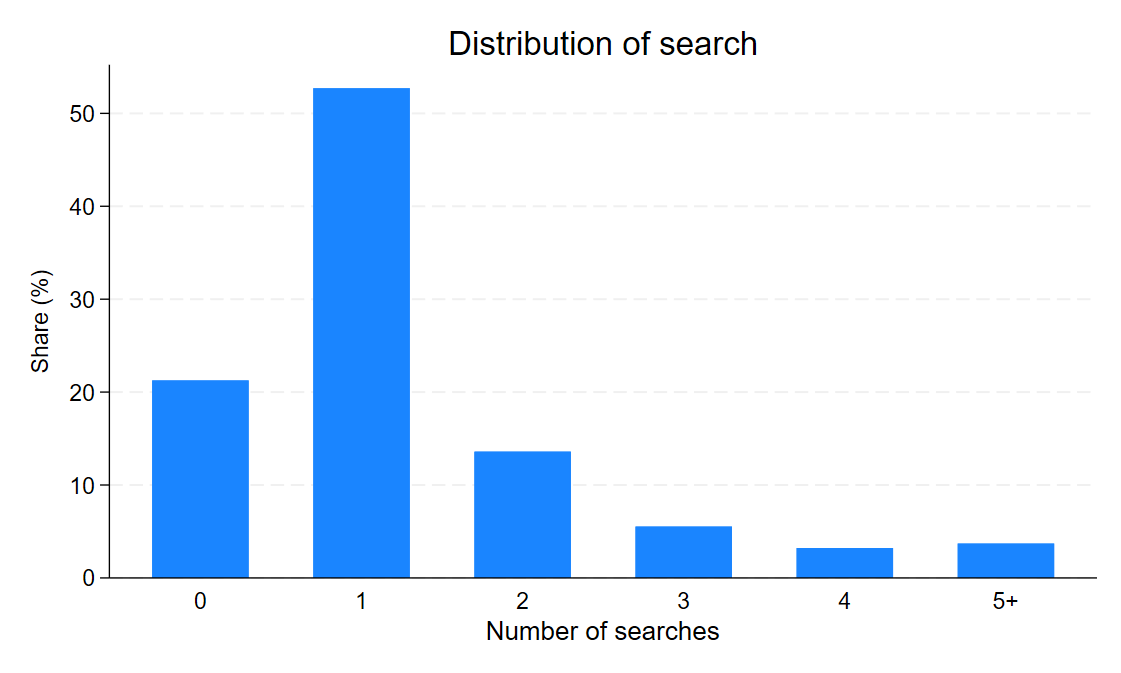
\includegraphics[width=0.49\textwidth]{../figures/IE3_dist_external_offers.png}
    \hfill % Pushes the images apart to fill the horizontal space
    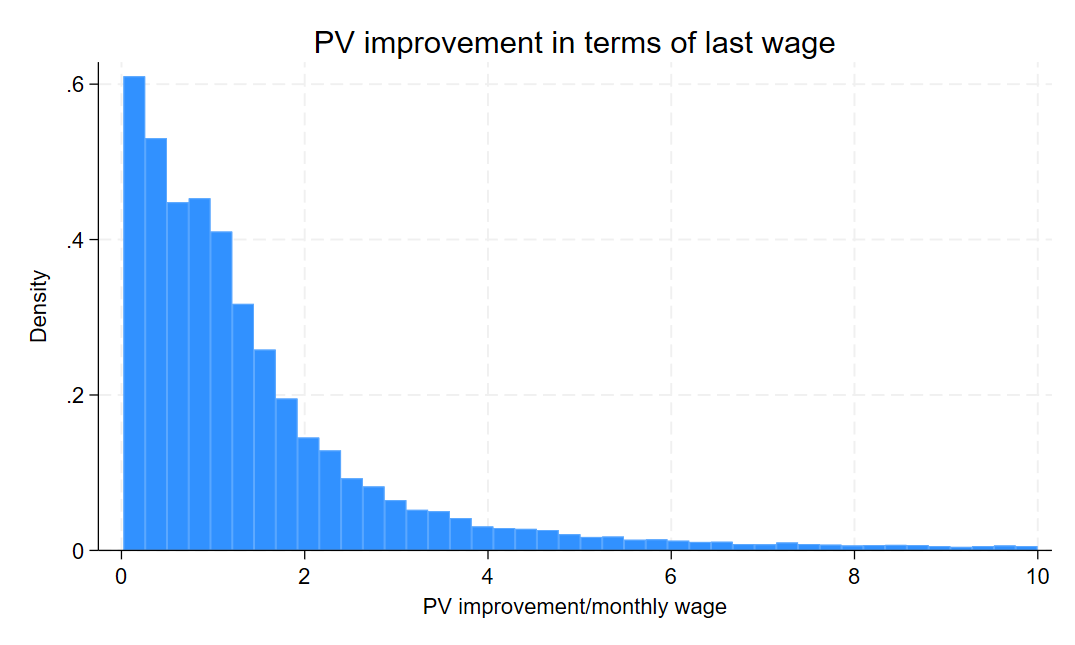
\includegraphics[width=0.49\textwidth]{../figures/IE3_offer_improvement_histogram.png}
    %\caption{Side-by-side figures.} % A single caption for both
    \label{fig:my-figures}
\end{figure}

\begin{itemize}
    \item   80\% of the purchases are through the aftermarket
\end{itemize}
\end{frame}



\begin{frame}{Literature}

\begin{itemize}
    \item Aftermarkets: \textcite{larsen_efficiency_2021, allen_search_2019}

    \item Competition in selection markets: \textcite{mahoney_imperfect_2017, cuesta_price_2018, cosconati_competing_2025}

    \item Selection in multiple dimensions: \textcite{finkelstein_adverse_2004} and Finkelstein and McGarry (2006).  
\end{itemize}
\end{frame}




%%%%%%%%%%%%%%%%%%%%%%%%%
% explicitly not link the annuities market with pensions because generates confusion 
\begin{frame}{Annuities in Chile: SCOMP}  \label{slide:setting}
    
    \begin{itemize}%[<+->]
   
\end{itemize} 
    \begin{itemize}%[<+->]
    \item SCOMP steps: 
    \begin{enumerate}
        \item Request of balance statement 
        \item Request for offers: asks for certain type of contracts (e.g. annuity)
        \item Insurers make offers (e.g. \$1000 per month)
        \item Retiree chooses one of the offers or asks for external offers

    \end{enumerate}

        \item External offers: bargaining and information disclosure
        %When offering insurers know 1. age, 2. amount of savings, 3. gender, 4. dependents. With external offers they learn your RUT(SSN): more information  
    

    \item Firms competition 1. financing cost 2. prediction algorithm 

    \item Profits of firm $j$: 
    \begin{align*}
    \pi_{ji}(F) = S_i-  \mathbb{E}^j_{T} \left[\sum_{t=1}^T\frac{F}{(1+r_j)^t}|x_i \right]
    \end{align*}
    % if it was only financing cost, it would be a monopoly
    \end{itemize}

     $S$: stock of savings, $F$: per period annuity payment, $x_i$: individual mortality factors
    
\end{frame}

%%%%%%%%%%%%%%%%%%%%%%%%%%%%%%%%%%%%%%

 \begin{frame}{Data} \label{slide:data}
\begin{itemize}
    \item SCOMP data at the individual level  
    \begin{itemize}
        \item Offers received, rejected and accepted 
        \item Total savings 
        \item Demographics: age and gender
    \end{itemize}
     \item Retirement insurance companies: risk ratings, \#  of intermediaries and their  locations.
\end{itemize}
\textbf{}

\textbf{}
\end{frame}

%%%%%%%%%%%%%%%%%%





%%%%%%%%%%%%%%%%%%%%%%%
\begin{frame}{Answer the question}
    \begin{itemize}
        \item Equilibrium model of search and bargaining 
        \begin{itemize}
            \ite
            \item Differentiated products   \hyperlink{slide:fig3}{\beamerbutton{Evidence}}
            \item Imperfect-assymmetric competition\hyperlink{slide:fig3}{\beamerbutton{Evidence}}
            \item 
        \end{itemize}
        \item 
    \end{itemize}

    \note{Diff products: if not the case then everyone would choose the highest offer
    
    Imperfect-assymmetric competition: the differences in market share can be due to preferences, but not so the differences in probability of even offering}
\end{frame}
%%%%%%%%%%%%%%%%%%%%%

\begin{frame}{Answer the question}\label{slide:fig3}    

Buyers do not always buy highest annuity. Average foregone value is 1.57 monthly wages.

\begin{figure}[H]
%\caption{}
\centering{}%
\begin{tabular}{cc}
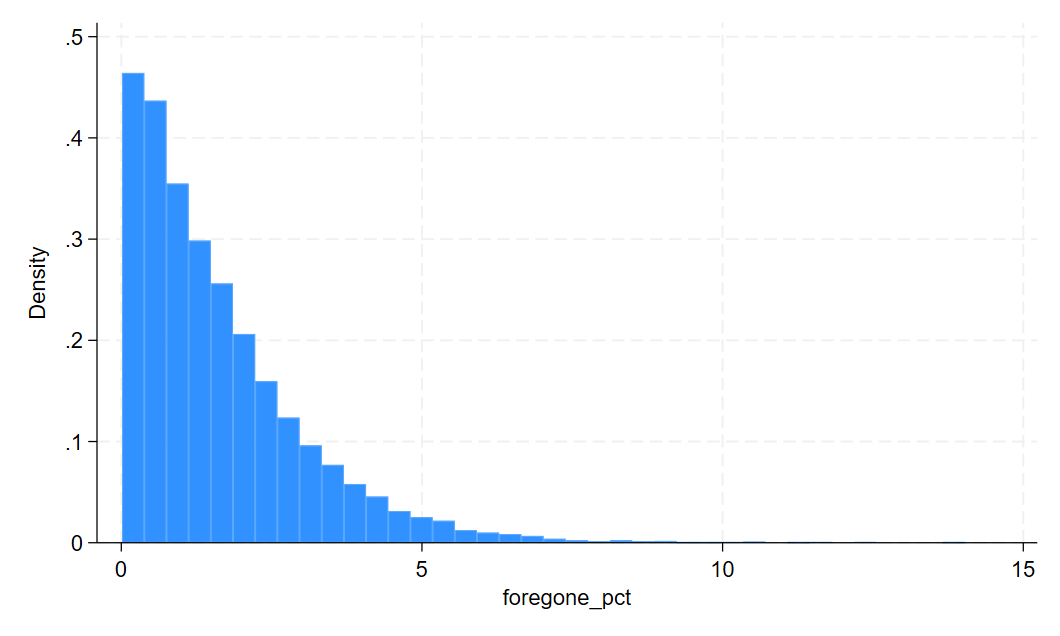
\includegraphics[scale=0.27]{../figures/IE3_foregone_hist.png}
\end{tabular}
\end{figure}
\end{frame}

 %%%%%%%





\begin{frame}{Answer the question}\label{slide:fig1}    

Firm specialization in groups
\begin{figure}[H]
%\caption{}
\centering{}%
\begin{tabular}{cc}
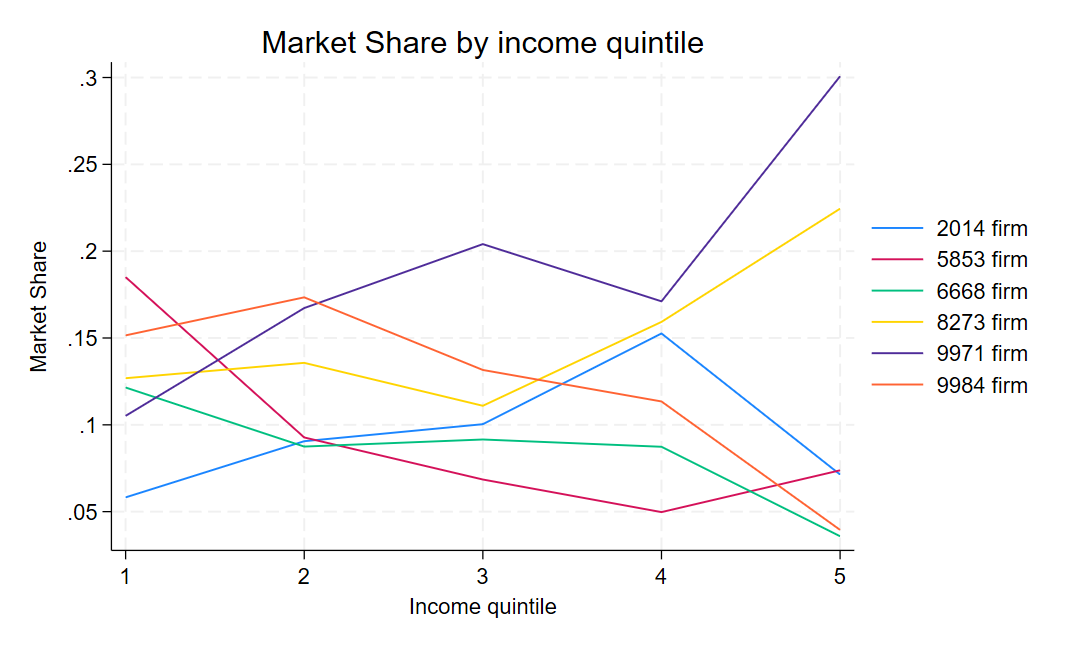
\includegraphics[scale=0.27]{../figures/IE3_supply_income_quintile.png}
\end{tabular}
\end{figure}
\end{frame}


\begin{frame}{Answer the question}\label{slide:fig2}    
\textcolor{red}{drop some firms, to cluttered}

\begin{figure}[H]
\caption{}
\centering{}%
\begin{tabular}{cc}
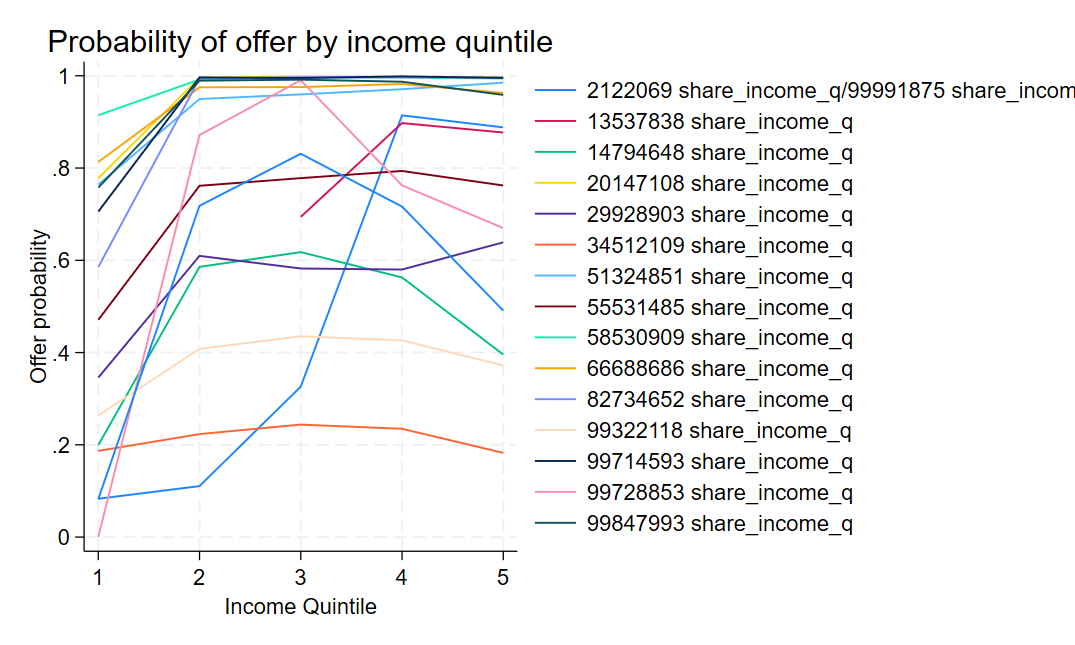
\includegraphics[scale=0.24]{../figures/IE3_supply_offerprob_income_q.png}
\end{tabular}
\end{figure}

Firms specialize on buyer types
\end{frame}

 





\end{document}